\vspace{200pt}

\section{Auswertung}
\label{sec:Auswertung}

\subsection{Stabilitätsbedingung}

Die maximal mögliche Resonatorlänge $L$ lässt sich für die verschiedenen
Spiegelkonfiguratioen aus der Stabilitätsbedingung

\vspace{-5pt}
\begin{equation}
    0 \leq g_1 g_2 \leq 1 \:, \qquad g = 1 - \frac{L}{r_i}
\end{equation}

bestimmen. Es werden zwei konkave Spiegel mit einem Krümmungsradius $r_\text{konkav} = \SI{1400}{\milli\meter}$
verwendet oder eine Kombination aus konkavem und planem Spiegel mit $r_\text{plan} \to \infty$.

\begin{figure}[H]
    \centering
    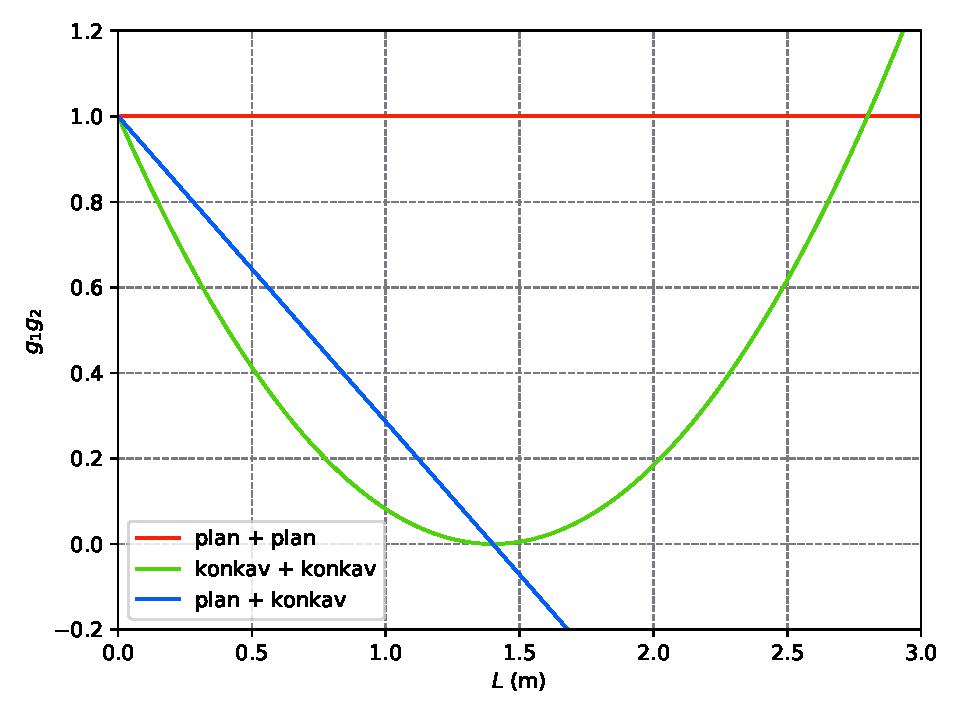
\includegraphics[scale=0.65]{content/g1g2.pdf}
    \vspace{-10pt}
    \caption{Stabilitätsparameter verschiedener Spiegelkonfigurationen planer und konkaver Spiegel mit einem Krümmungsradius
    von $r_\text{konkav} = \SI{1400}{\milli\meter}$.}
    \label{fig:stab}
\end{figure}

Die Stabilitätsparameter der verschiedenen Konfigurationen in Abhängigkeit der Resonatorlänge $L$ 
sind dabei in Abbildung \ref{fig:stab} dargestellt.
Für zwei plane Spiegel verläuft $g_1 g_2 = 1$ konstant, während $g_1 g_2$ für die Kombination eine Gerade 
beschreibt. Sie erfüllt die Stabilitätsbedingung für $0 \leq L \leq r_\text{konkav}$. Für
die beiden konkaven Spiegel verläuft $g_1 g_2$ parabelförmig und die Bedingung ist für  $0 \leq L \leq 2 \cdot r_\text{konkav}$
erfüllt. Es ergeben sich damit theoretisch die beiden maximalen Resonatorlängen

\vspace{-15pt}
\begin{align*}
    \text{  plan + konkav:} \qquad L_\text{pk,theo} &= \SI{1.4}{\meter} \: ,\\
    \text{konkav + konkav:} \qquad L_\text{kk,theo} &= \SI{2.8}{\meter}
\end{align*}

und aus der Tabelle \ref{tab:gg} und Abbildung \ref{fig:gg} ergeben sich die gemessenen Längen

\vspace{-15pt}
\begin{align*}
    \text{  plan + konkav:} \qquad L_\text{pk,exp} &= \SI{0.834}{\meter} \: ,\\
    \text{konkav + konkav:} \qquad L_\text{kk,exp} &= \SI{1.003}{\meter} \: .
\end{align*}

\begin{table}[H]
    \centering
    \footnotesize
    \caption{Intensitätsmesswerte $I(L)$ der beiden Resonatorkonfigurationen.}
    \label{tab:gg}
    \sisetup{table-format=2.1}
    \begin{tabular}{r r r r | r r r r}
    \toprule
    $L_{pk} \;/\; \si{\centi\meter}$ & $I_{pk} \;/\; \si{\milli\watt}$ & 
    $L_{pk} \;/\; \si{\centi\meter}$ & $I_{pk} \;/\; \si{\milli\watt}$ &
    $L_{kk} \;/\; \si{\centi\meter}$ & $I_{kk} \;/\; \si{\milli\watt}$ & 
    $L_{kk} \;/\; \si{\centi\meter}$ & $I_{kk} \;/\; \si{\milli\watt}$ \\
    \midrule
    55,8 & 3,05 & 72,5 & 0,98 & 69,2 & 4,85 &  87,6 & 6,10 \\
    58,2 & 1,80 & 75,4 & 2,50 & 72,1 & 4,28 &  91,0 & 5,45 \\
    60,9 & 1,52 & 79,0 & 1,20 & 76,0 & 4,50 &  92,7 & 4,90 \\
    65,0 & 2,26 & 81,7 & 0,80 & 80,2 & 4,20 &  95,5 & 4,40 \\
    68,4 & 1,37 & 83,4 & 1,84 & 84,8 & 5,80 &  98,2 & 2,60 \\  
         &      &      &      &      &      & 100,3 & 2,10 \\
    \bottomrule
    \end{tabular}
\end{table}

\begin{figure}[H]
    \centering
    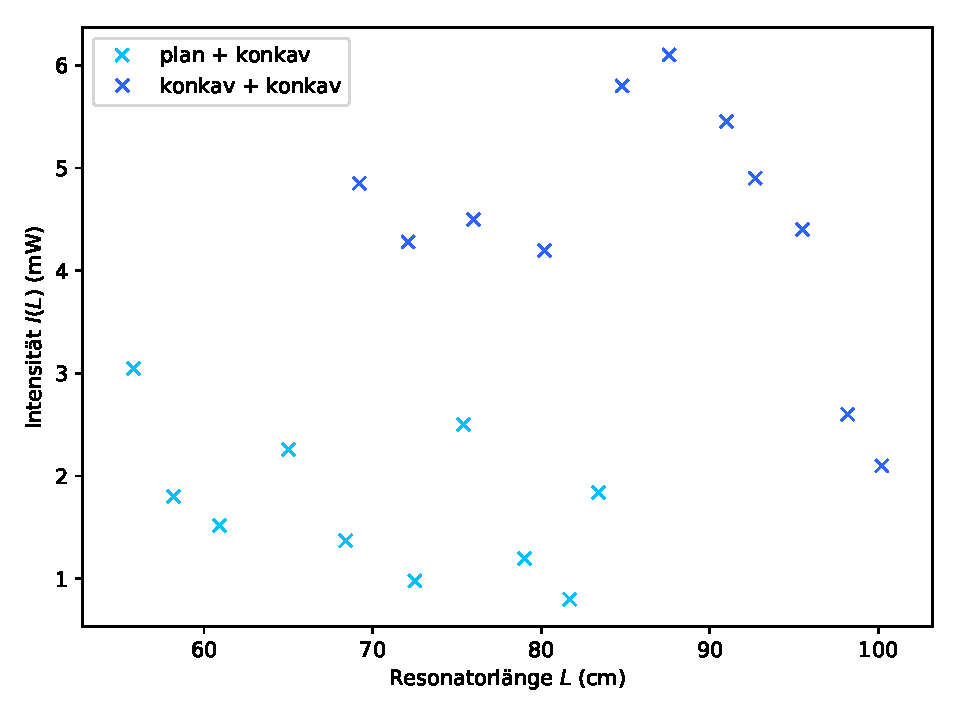
\includegraphics[scale=0.65]{content/gg.pdf}
    \vspace{-10pt}
    \caption{Intensitätsverteilung $I(L)$ der beiden Resonatorkonfigurationen.}
    \label{fig:gg}
\end{figure}



\subsection{Wellenlänge}

Die Wellenlänge kann durch Analyse verschiedener Gitterinterferenzspektren bestimmt werden.
Dazu sind die Abstände $d_n$ der $n$-ten Maxima zur optischen Achse für vier verschiedene
Gitter mit den Gitterkonstanten 

\vspace{-5pt}
\begin{equation*}
    g_1 = \SI{80}{\milli\meter\tothe{-1}} \, , \quad g_2 = \SI{100}{\milli\meter\tothe{-1}} \, , \quad 
    g_3 = \SI{600}{\milli\meter\tothe{-1}} \, , \quad g_4 = \SI{1200}{\milli\meter\tothe{-1}}
\end{equation*}

in der Tabelle \ref{tab:mess} aufgelistet. Die Abstände zwischen Gitter und Schirm sind dabei

\vspace{-5pt}
\begin{equation*}
    l_1=l_2=l_3 = \SI{76}{\centi\meter}\: , \qquad l_4 = \SI{25}{\centi\meter}\: .
\end{equation*}

\begin{table}[H]
    \centering
    \footnotesize
    \caption{Messwerte der Abstände $d_n$ der $n$-ten Interferenzmaxima zur optischen Achse für vier verschiedene optische Gitter.}
    \label{tab:mess}
    \sisetup{table-format=2.1}
    \begin{tabular}{c | r r r r}
    \toprule
    $n$ & $d_{n,g_1} \;/\; \si{\centi\meter}$ & $d_{n,g_2} \;/\; \si{\centi\meter}$ & $d_{n,g_3} \;/\; \si{\centi\meter}$ &
    $d_{n,g_4} \;/\; \si{\centi\meter}$ \\
    \midrule
         -6 & 24,7 & 32,3 & -    & -    \\
         -5 & 20,2 & 26,1 & -    & -    \\
         -4 & 15,9 & 20,3 & -    & -    \\
         -3 & 11,8 & 14,8 & -    & -    \\
         -2 &  7,8 &  9,7 & -    & -    \\
         -1 &  3,9 &  4,8 & 32,5 & 30,3 \\
          0 &  0,0 &  0,0 &  0,0 &  0,0 \\
          1 &  4,0 &  4,7 & 31,3 & 29,0 \\
          2 &  8,0 &  9,6 & -    & -    \\
          3 & 12,0 & 14,5 & -    & -    \\
          4 & 16,0 & 19,5 & -    & -    \\
          5 & 20,1 & 24,7 & -    & -    \\
          6 & 24,3 & 30,2 & -    & -    \\
          7 & 28,8 & 35,9 & -    & -    \\
          8 & 33,6 & -    & -    & -    \\
    \bottomrule
    \end{tabular}
\end{table}

Die Wellenlängen können mithilfe der Ordnung $n$, den Gitterkonstanten $g_i$ und Abständen $l_i$
zwischen Gittern und Schirm bestimmt werden als

\vspace{-5pt}
\begin{equation}
    \lambda = \frac{\text{sin}\left(\text{tan}\left(\frac{d_n}{l}\right)\right)}{n \cdot g}\: .
\end{equation}

Für angenommene Messungenauigkeiten von $\sigma_{d_n} = \SI{0.1}{\centi\meter}$ 
und $\sigma_l = \SI{2}{\centi\meter}$
resultiert dann eine gemittelte Wellenlänge von

\vspace{-5pt}
\begin{equation*}
    \bar{\lambda} = \SI{658 +- 34}{\nano\meter} \: .
\end{equation*}

\subsection{Transversale Moden}
\subsubsection{TEM$_{00}$-Mode}

Die Messdaten der senkrecht zur optischen Achse gemessene Intensitätsverteilung
der TEM$_{00}$-Mode sind in Tabelle \ref{tab:TEM00} aufgelistet und können
mittels der Funktion \textit{scipy.optimize.curve\_fit} aus der Python-Bibliothek SkiPy
mit der theoretischen Gaußverteilung 

\vspace{-5pt}
\begin{equation}
    I_{00}(r) = I_0 \cdot \text{exp}\left(-\frac{(r-r_0)^2}{2 \omega^2}\right)
\end{equation}

approximiert werden. Es ergeben sich die Fitparameter

\vspace{-15pt}
\begin{align*}
    I_0 &= \SI{10.38 +- 0.14}{\micro\watt} \: ,\\
    r_0 &= \SI{0.51 +- 0.10}{\milli\meter} \: , \\
    \omega &= \SI{6.82 +- 0.11}{\milli\meter} \: .
\end{align*}

\begin{table}[H]
    \centering
    \footnotesize
    \caption{Messwerte der Intensität $I(r)$ der TEM$_{00}$-Mode abhängig vom Modenmittenabstand $r$.}
    \label{tab:TEM00}
    \sisetup{table-format=2.1}
    \begin{tabular}{r r | r r | r r}
    \toprule
    $r \;/\; \si{\milli\meter}$ & $I \;/\; \si{\micro\watt}$ & $r \;/\; \si{\milli\meter}$ & $I \;/\; \si{\micro\watt}$
    & $r \;/\; \si{\milli\meter}$ & $I \;/\; \si{\micro\watt}$ \\
    \midrule
        -13 & 1,0 & -3 &  9,6 &  7 & 6,7 \\
        -12 & 1,5 & -2 &  9,7 &  8 & 6,0 \\
        -11 & 2,1 & -1 & 10,4 &  9 & 5,0 \\
        -10 & 2,6 &  0 & 11,0 & 10 & 4,2 \\
         -9 & 3,7 &  1 & 10,3 & 11 & 3,4 \\
         -8 & 4,9 &  2 & 10,1 & 12 & 2,6 \\
         -7 & 5,8 &  3 &  8,8 & 13 & 2,3 \\
         -6 & 6,7 &  4 &  8,5 & 14 & 1,7 \\
         -5 & 7,8 &  5 &  7,9 & 15 & 1,3 \\
         -4 & 8,4 &  6 &  7,3 \\
    \bottomrule
    \end{tabular}
\end{table}


\vspace{-15pt}

\begin{figure}[H]
    \centering
    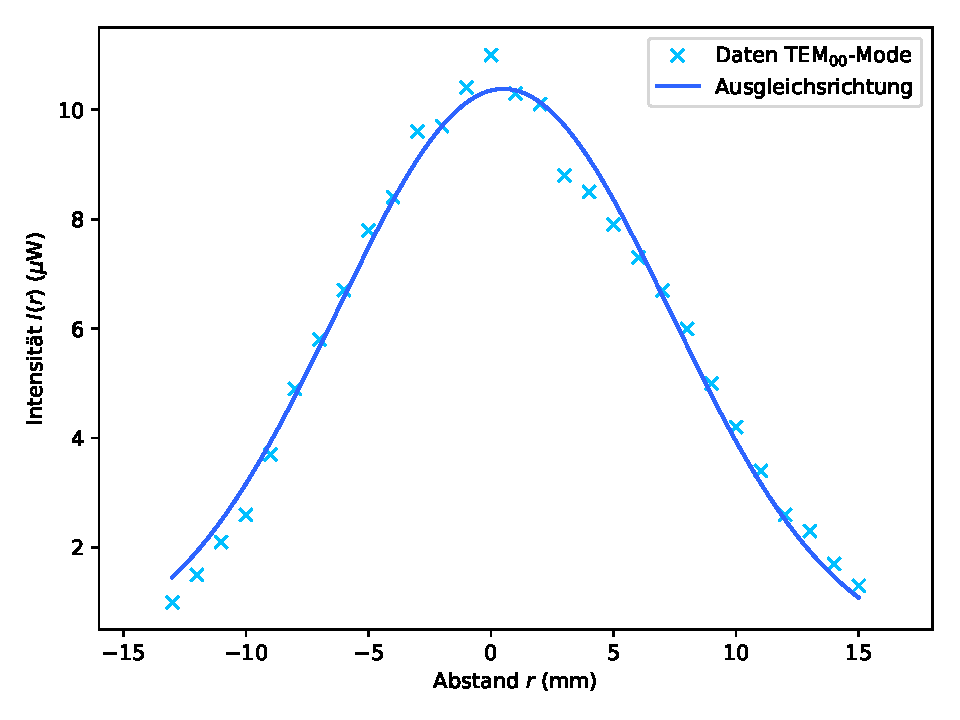
\includegraphics[scale=0.65]{content/TEM00.pdf}
    \vspace{-10pt}
    \caption{Intensitätsverteilung $I(r)$ der TEM$_{00}$-Mode für verschiedene Abstände $r$ von der Modenmitte.}
    \label{fig:TEM00}
\end{figure}

\subsubsection{TEM$_{01}$-Mode}

Für die in Tabelle \ref{tab:TEM01} aufgelisteten Messdaten der TEM$_{01}$-Mode
wird unter Berücksichtigung eines Offset $I_\text{off} = \SI{0.1}{\micro\watt}$ gleich verfahren 
und die Approximation erfolgt mit der Funktion

\vspace{-5pt}
\begin{equation}
    I_{01}(r) = I_0 \cdot \frac{8(r-r_0)^2}{\omega^2} \cdot \text{exp}\left(-\frac{2(r-r_0)^2}{\omega^2}\right) + I_\text{off} \: .
\end{equation}

Es ergeben sich die Fitparameter

\vspace{-15pt}
\begin{align*}
    I_0 &= \SI{0.145 +- 0.010}{\micro\watt} \: , \\
    r_0 &= \SI{0.6 +- 0.4}{\milli\meter}\: , \\
    \omega &= \SI{8.2 +- 0.4}{\milli\meter} \: .
\end{align*}

\begin{table}[H]
    \centering
    \footnotesize
    \caption{Messwerte der Intensität $I(r)$ der TEM$_{01}$-Mode abhängig vom Modenmittenabstand $r$.}
    \label{tab:TEM01}
    \sisetup{table-format=2.1}
    \begin{tabular}{r r | r r | r r}
    \toprule
    $r \;/\; \si{\milli\meter}$ & $I \;/\; \si{\micro\watt}$ & $r \;/\; \si{\milli\meter}$ & $I \;/\; \si{\micro\watt}$
    & $r \;/\; \si{\milli\meter}$ & $I \;/\; \si{\micro\watt}$ \\
    \midrule
        -13 & 0,17 & -3 & 0,20 &  7 & 0,38 \\
        -12 & 0,27 & -2 & 0,17 &  8 & 0,66 \\
        -11 & 0,39 & -1 & 0,13 &  9 & 0,74 \\
        -10 & 0,50 &  0 & 0,12 & 10 & 0,72 \\
         -9 & 0,64 &  1 & 0,10 & 11 & 0,58 \\
         -8 & 0,56 &  2 & 0,11 & 12 & 0,40 \\
         -7 & 0,51 &  3 & 0,13 & 13 & 0,20 \\
         -6 & 0,40 &  4 & 0,20 & 14 & 0,18 \\
         -5 & 0,37 &  5 & 0,27 \\
         -4 & 0,27 &  6 & 0,31 \\
    \bottomrule
    \end{tabular}
\end{table}

\vspace{-15pt}

\begin{figure}[H]
    \centering
    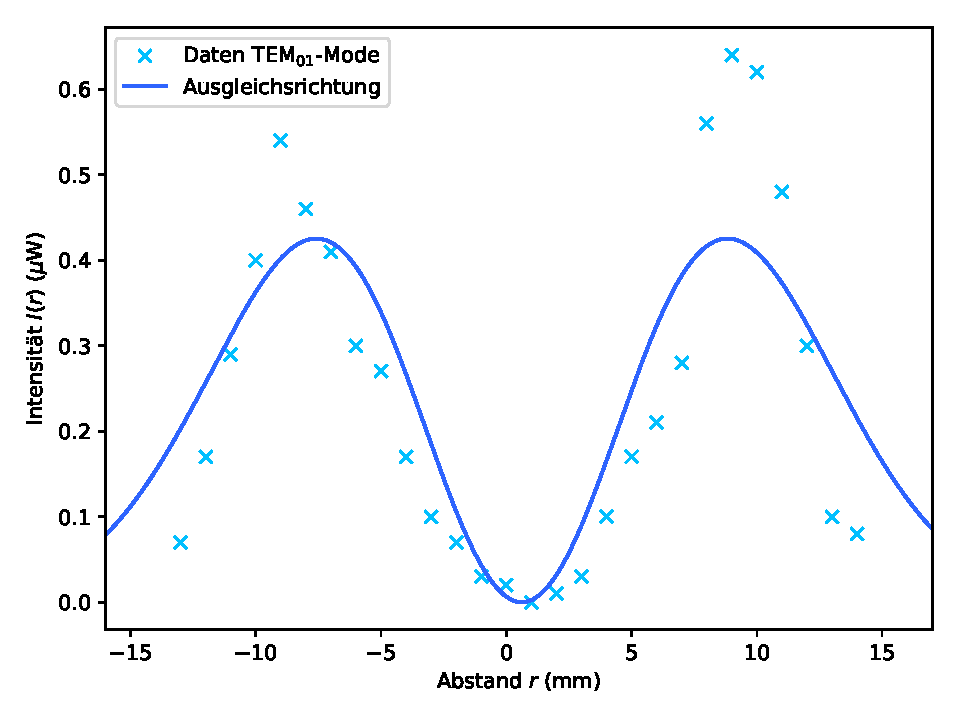
\includegraphics[scale=0.65]{content/TEM01.pdf}
    \vspace{-10pt}
    \caption{Intensitätsverteilung $I(r)$ der TEM$_{01}$-Mode für verschiedene Abstände $r$ von der Modenmitte.}
    \label{fig:TEM01}
\end{figure}

\subsection{Polarisation}

Die Daten der Intensitätsverteilung, die in Abhängigkeit des Polarisationswinkels $\phi$ in 
$\SI{10}{\degree}$-Schritten gemessen werden, sind in Tabelle \ref{tab:pol} aufgelistet.
Eine Ausgleichsrechnung der Form 

\vspace{-15pt}
\begin{equation}
    I_P(\phi) = I_0 \cdot \text{cos}^2 \left((\phi  + \phi_0)\cdot \frac{2\pi}{\SI{360}{\degree}}\right)
\end{equation}

ergibt die Parameter

\vspace{-15pt}
\begin{align*}
    I_0 &= \SI{0.904 +- 0.006}{\milli\watt}\: , \\ 
    \phi_0 &= \SI{80.64 +- 0.31}{\degree} \: .
\end{align*}

\begin{table}[H]
    \centering
    \footnotesize
    \caption{Messwerte der Intensität $I(\phi)$ abhängig vom Polarisationswinkel $\phi$.}
    \label{tab:pol}
    \sisetup{table-format=2.1}
    \begin{tabular}{r r | r r | r r}
    \toprule
    $\phi \;/\; \si{\degree}$ & $I \;/\; \si{\milli\watt}$ & $\phi \;/\; \si{\degree}$ & $I \;/\; \si{\milli\watt}$
    & $\phi \;/\; \si{\degree}$ & $I \;/\; \si{\milli\watt}$ \\
    \midrule
         0 & 0,02 & 120 & 0,76 & 240 & 0,54 \\
        10 & 0,00 & 130 & 0,63 & 250 & 0,71 \\
        20 & 0,03 & 140 & 0,48 & 260 & 0,82 \\
        30 & 0,10 & 150 & 0,35 & 270 & 0,89 \\
        40 & 0,21 & 160 & 0,20 & 280 & 0,91 \\
        50 & 0,36 & 170 & 0,09 & 290 & 0,87 \\
        60 & 0,53 & 180 & 0,02 & 300 & 0,82 \\
        70 & 0,67 & 190 & 0,00 & 310 & 0,68 \\
        80 & 0,79 & 200 & 0,03 & 320 & 0,54 \\
        90 & 0,88 & 210 & 0,11 & 330 & 0,39 \\
       100 & 0,97 & 220 & 0,23 & 340 & 0,23 \\
       110 & 0,85 & 230 & 0,39 & 350 & 0,10 \\
    \bottomrule
    \end{tabular}
\end{table}

\vspace{-15pt}

\begin{figure}[H]
    \centering
    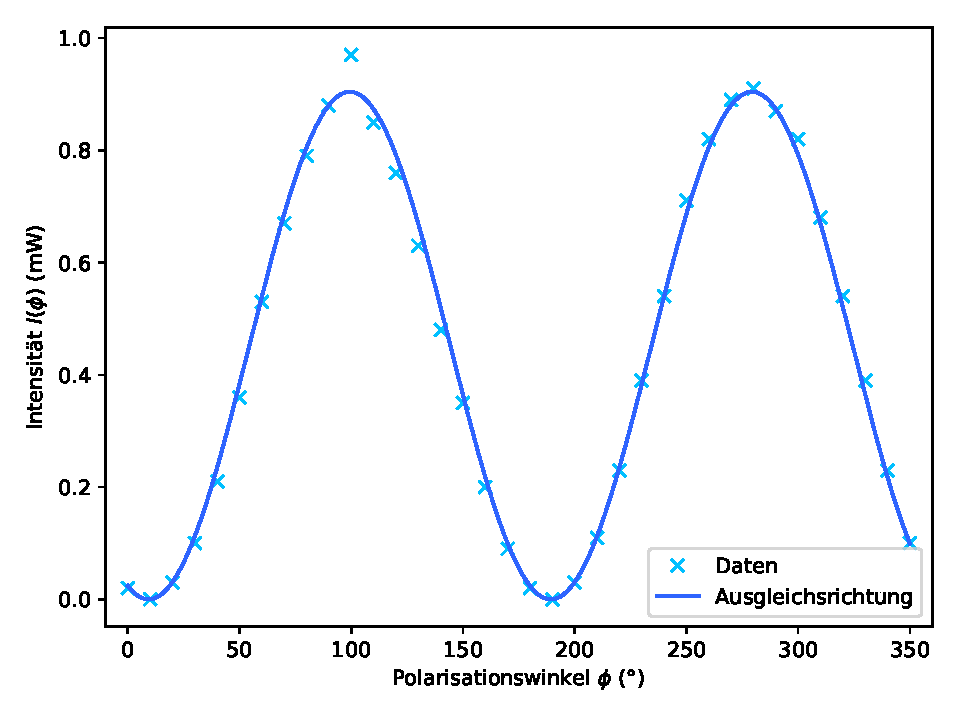
\includegraphics[scale=0.65]{content/pol.pdf}
    \vspace{-10pt}
    \caption{Intensitätsverteilung $I(\phi)$ für verschiedene Polarisationswinkel $\phi$.}
    \label{fig:pol}
\end{figure}

\subsection{Longitudinale Moden}

Für verschiedene Resonatorlängen $L$ sind die Frequenzen der fouriertransformierten Peaks der
jeweils ersten drei longitudinalen Moden in Tabelle \ref{tab:long} aufgelistet.
Für drei Resonatorlängen $L$ ergeben sich die Abstände der Moden zu

\vspace{-15pt}
\begin{align*}
    L &= \SI{ 69.2}{\centi\meter}: & \Delta f_{1,2} &= \SI{217}{\mega\hertz}\, , & \Delta f_{2,3 } &= \SI{214}{\mega\hertz}\, , & \bar{\Delta f} &= \SI{215.5}{\mega\hertz}\, , \\  
    L &= \SI{ 84.8}{\centi\meter}: & \Delta f_{1,2} &= \SI{176}{\mega\hertz}\, , & \Delta f_{2,3 } &= \SI{173}{\mega\hertz}\, , & \bar{\Delta f} &= \SI{174.5}{\mega\hertz}\, , \\  
    L &= \SI{100.3}{\centi\meter}: & \Delta f_{1,2} &= \SI{146}{\mega\hertz}\, , & \Delta f_{2,3 } &= \SI{154}{\mega\hertz}\, , & \bar{\Delta f} &= \SI{150}{\mega\hertz}\, .  
\end{align*}

Mit der Lichtgeschwindigkeit $c = \SI{299 792 458}{\meter\per\second}$ ergeben sich nach  

\vspace{-5pt}
\begin{equation}
    \Delta f = \frac{c}{2 \cdot L}
\end{equation}

die theoretischen Modendifferenzen zu

\vspace{-15pt}
\begin{align*}
    L &= \SI{ 69.2}{\centi\meter}: & \Delta f_\text{theo} &= \SI{216.61}{\mega\hertz}\, , \\  
    L &= \SI{ 84.8}{\centi\meter}: & \Delta f_\text{theo} &= \SI{176.76}{\mega\hertz}\, , \\  
    L &= \SI{100.3}{\centi\meter}: & \Delta f_\text{theo} &= \SI{149.46}{\mega\hertz}\, .  
\end{align*}

Die Doppler-Verbreiterung des Neon-Übergangs berechnet sich nach \cite[S.49]{spektro}
unter Verwendung der allgemeinen Gaskonstante $R$ zu

\vspace{-5pt}
\begin{equation}
    \partial f_D = \frac{2f_0}{c} \sqrt{\frac{2RT\: \text{ln}(2)}{M}} 
    = \num{7.16e-7}\sqrt{\frac{\si{\gram\per\mol}}{\si{\kelvin}}} \cdot f_0 \cdot \sqrt{\frac{T}{M}}
    = \SI{1.314}{\giga\hertz} = \SI{1314}{\mega\hertz}
\end{equation}

mit der Laserfrequenz 

\vspace{-5pt}
\begin{equation}
    f_0 = \frac{\lambda}{c} = \SI{4.74e5}{\giga\hertz}
\end{equation}

und der Molmasse
$M = \SI{20}{\gram\per\mol}$ bei Raumtemperatur $T = \SI{300}{\kelvin}$.
Die Doppler-Verbreiterung entspricht mit steigender Resonatorlänge etwa dem $6$-, $7,5$-, und $9$-fachen der 
gemittelten Modenabstände $\bar{\Delta f}$.

\begin{table}[H]
    \centering
    \footnotesize
    \caption{Messwerte der jeweils ersten drei Peakfrequenzen $f_i\:, \; i = 1,2,3$ 
    abhängig von der Resonatorlänge $L$.}
    \label{tab:long}
    \sisetup{table-format=2.1}
    \begin{tabular}{r r | r r | r r}
    \toprule
    $L \;/\; \si{\centi\meter}$ & $f_i \;/\; \si{\mega\hertz}$ & 
    $L \;/\; \si{\centi\meter}$ & $f_i \;/\; \si{\mega\hertz}$ & 
    $L \;/\; \si{\centi\meter}$ & $f_i \;/\; \si{\mega\hertz}$ \\
    \midrule
         69,2 & 218 & 84,8 & 180 &  95,5 & 158 \\
              & 435 &      & 356 &       & 315 \\
              & 649 &      & 529 &       & 473 \\
         72,1 & 210 & 91,0 & 169 & 100,3 & 154 \\
              & 416 &      & 330 &       & 300 \\
              & 623 &      & 495 &       & 454 \\
        
    \bottomrule
    \end{tabular}
\end{table}